\chapter{Background \& Related Work}
\section{Background}
In this section, I will list all technologies that are used in this project along with discussing other papers which were trying to address security with IoT devices by also trying to include blockchain technology.
\subsection{MQTT}
When designing architecture with the main target being communication of many (even couple of thousands a second) clients constantly exchanging data, scalability and availability needs to be kept in mind. The first and obvious solution would be to directly connect data consumers and data produces, by making them communicate in Peer-to-Peer fashion, removing the need for any extra infrastructure. This might work perfectly fine with small systems (disregarding issues such as dynamic DNS or static IP), but as number of clients requesting access to data increases, the total capacity of the sensor would eventually be capped - since IoT usually are of limited power and computation capacity. Imagine a scenario where a single temperature sensor constantly getting bombarded with requests for current readings, it might be able to cope up to 5 incoming requests every second, everything else would cause malfunction or significantly slower response times.

Then there is also an issue of security. By allowing clients to connect to our IoT devices, we are opening an extra attack vector. What if the client doesn't want to only access the temperature readings, but perhaps inject a worm which would intercept other sensors (such as cameras). Recently ``smart nannies'', responsible for alerting the parents when the child is crying and also relieving the adults from having to be constantly nearby, gained popularity. A direct camera feed could be accesses via smart phone, no matter where. This eventually led to exploitation, as it was found that many of those devices were vulnerable to remote access by third parties\cite{pultarova2016webcam}.

MQTT aims to address those issues and not only, by moving the communication to a separate client, which operates on publish-subscribe fashion. This would mean that IoT devices only have to publish information that is available to them (e.g. temperature readings), allowing to completely remove remote access, effectively removing this particular attack threat. Furthermore, the MQTT brokers can be further placed behind load balancers and such to further enhance their availability.
\begin{figure}[h]
    \centering
    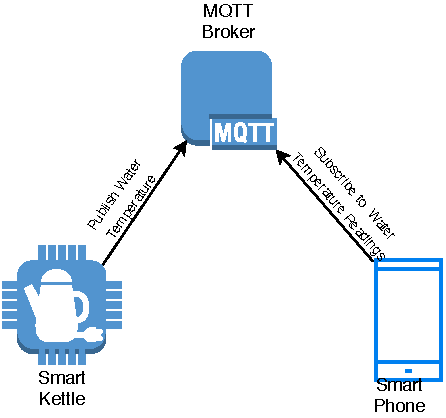
\includegraphics[width=0.5\textwidth]{mqtt_demo}
    \caption{MQTT Broker Architecture}
    \label{fig:mqtt}
\end{figure}
In short, MQTT, fully expanded to Message Queueing Telemetry Transport is an open protocol, certified by OASIS and ISO\cite{banks2019mqtt}, responsible for publisher-subscriber architecture. It's important to point out that MQTT is not a piece of software or a server, but rather a set of standards defining what potential clients can expect (what kind of responses and data) while connection to brokers following the standard. Figure \ref{fig:mqtt} briefly shows how MQTT-compatible broker can relay information between clients. Smart Phone and Smart Kettle don't have to be online at the same time in order to receive information, nor Smart Phone is even permitted to initiate direct connection to Smart Kettle
\section{Related Work}
This section will talk about other scientific papers which had similar goal in mind, by combining  blockchain technologies with IoT or even MQTT brokers.

